\documentclass[a4paper, 12pt]{article}
\usepackage[top=2cm, left=2cm, right=1cm, bottom=1cm]{geometry}
\usepackage{tikz}
\usepackage[utf8]{inputenc}

\begin{document}
	\section{Example Figures}
	
	\begin{figure}[h!]
		\centering
		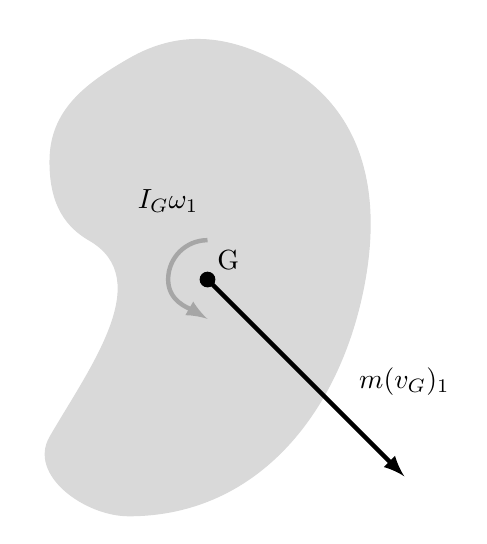
\begin{tikzpicture}
			\filldraw[gray!30] (-1,-3) to[out=0, in=260] (2,0) to[out=80, in=330] (1,2.7) to[out=150, in=30] (-1,2.8) to[out=210,in=90] (-2,1.5) to[out=270, in=150] (-1.5,.5) to[out=330,in=60] (-2,-2) to[out=240,in=180] (-1,-3);
			%\draw[help lines] (-2,-3) grid (2,3);
			
			\fill[black] (0,0) node[above right]{G} circle (1mm); 
			\draw[->,ultra thick,>=latex,gray!70] (0,0.5) to[out=180, in=90] (-.5,0) to[out=270,in=150] (0,-.5);
			\draw[->,ultra thick,>=latex] (0,0) -- (2.5,-2.5);
			\draw (-.5,1) node{$I_{G}\omega_{1}$};
			\draw (2.5,-1.3) node{$m(v_{G})_{1}$};
		\end{tikzpicture}
		\caption{Motion quantity diagram}
	\end{figure}

	\begin{figure}[h!]
		\centering
		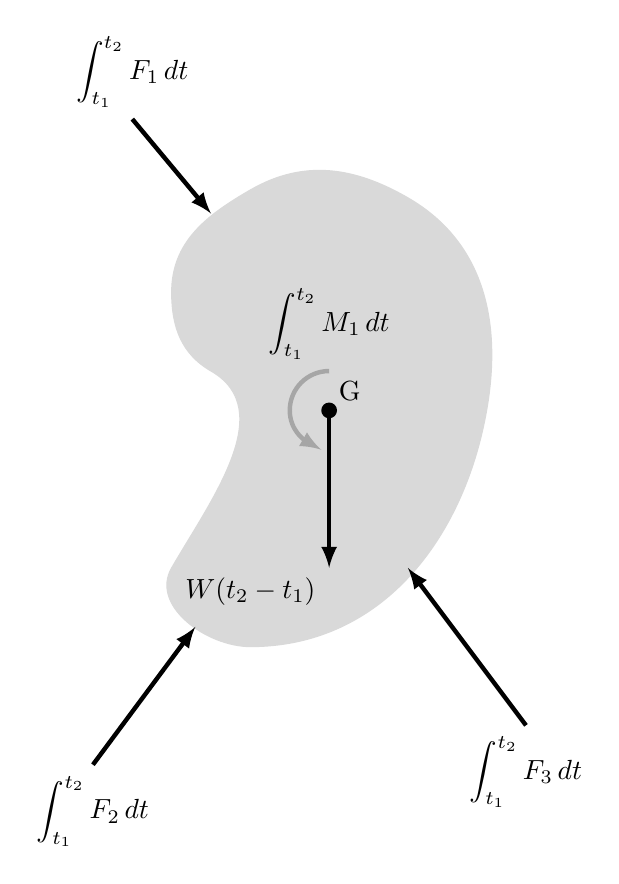
\begin{tikzpicture}
		\filldraw[gray!30] (-1,-3) to[out=0, in=260] (2,0) to[out=80, in=330] (1,2.7) to[out=150, in=30] (-1,2.8) to[out=210,in=90] (-2,1.5) to[out=270, in=150] (-1.5,.5) to[out=330,in=60] (-2,-2) to[out=240,in=180] (-1,-3);
		%\draw[help lines,dashed] (-2,-3) grid (2,3);
		
		\fill[black] (0,0) node[above right]{G} circle (1mm); 
		\draw[->,ultra thick,>=latex,gray!70] (0,0.5) to[out=180, in=90] (-.5,0) to[out=270,in=150] (-.1,-.5);
		
		\draw (0,1.1) node{$\displaystyle\int_{t_{1}}^{t_{2}}M_{1}\,dt$};
		
		\draw[->,ultra thick,>=latex] (2.5,-4) node[below]{$\displaystyle\int_{t_{1}}^{t_{2}}F_{3}\,dt$}-- (1,-2) ;
		\draw[->,ultra thick,>=latex] (-3,-4.5) node[below]{$\displaystyle\int_{t_{1}}^{t_{2}}F_{2}\,dt$} -- (-1.7,-2.75);
		\draw[->,ultra thick,>=latex] (-2.5,3.7) node[above]{$\displaystyle\int_{t_{1}}^{t_{2}}F_{1}\,dt$}-- (-1.5,2.5);
		\draw[->,ultra thick,>=latex] (0,0) -- (0,-2);
        \draw (-1,-2.3) node{$W(t_{2}-t_{1})$};
		\end{tikzpicture}
		\caption{Impulse diagram}
	\end{figure}
\end{document}